\documentclass{article}
\usepackage{amsmath,amsfonts,graphicx,fullpage,comment}

\newcommand{\HRule}{\rule{\linewidth}{0.5mm}}
\begin{document}

\begin{titlepage}
 
\begin{center}
 
\textsc{\LARGE Homework 1}\\[1.5cm]
 
\textsc{\Large Computational Math}\\[0.5cm]
 
 
 
\HRule \\[2cm]
 
% Author and supervisor
\begin{minipage}{0.4\textwidth}
\begin{flushleft} \large
\emph{Author:}\\
Mikola Lysenko
\end{flushleft}
\end{minipage}
 
\vfill
 
% Bottom of the page
{\large \today}
 
\end{center}
 
\end{titlepage}


\paragraph{1}
Let $\varphi(x) = e^{\sin{x} \cos{x}}$.  To verify that BC1 and BC2 are satisified, we establish the stronger condition that $\varphi$ is periodic:
\[ \varphi(x + 2 \pi) = e^{\sin(x + 2\pi)} e^{\cos (x + 2\pi)} = e^{\sin(x)} e^{\cos(x)} = \varphi(x) \]
Which trivially implies BC1.  To check BC2 we observe:
\begin{eqnarray*}
\varphi_x(x + 2\pi) & = & \mathop{\lim }\limits_{\delta \to 0} \frac{ \varphi(x + \delta + 2 \pi) - \varphi(x + 2 \pi) } { \delta } \\
& = & \mathop{\lim }\limits_{\delta \to 0} \frac{ \varphi(x + \delta) - \varphi(x) } { \delta } \\
& = & \varphi_x(x)
\end{eqnarray*}
And thus BC2 is satisified as well.  Finally, we verify ODE via direct substitution.  Taking partial derivatives we find:
\[ \varphi_{xx}(x) = \left( \left( \cos(x) - \sin(x) \right)^2 - \left( \sin(x) + \cos(x) \right) \right)\varphi(x) \]
So ODE expands to:
\[ \left( \left( \cos(x) - \sin(x) \right)^2 - \left( \sin(x) + \cos(x) \right) + \sin(x) + \cos(x) + 2 \sin(x) \cos(x) - 1 \right) \varphi(x) = 0 \]
Regrouping terms in the left subexpression gives the following elementary trig identities:
\begin{eqnarray*}
\left( \sin(x) + \cos(x) \right) - \left( \sin(x) + \cos(x) \right) & = & 0 \\
\left( \cos(x) - \sin(x) \right)^2  + 2 \sin(x) \cos(x) - 1 & = & 0
\end{eqnarray*}
Therefore the solution is exact.

\paragraph{2}
First, observe that all $2\pi$-periodic functions satisfy BC1 and BC2 (by the argument from exercise 1), and thus the approximation trivally satisifies the boundary conditions.  Now we make the following observation; the Galerkin solution ...
\[ \varphi(x) \approx a_0 + \sum \limits_{n=1}^N \left( a_n \cos(nx) + b_n \sin(nx) \right) \]
... may be written as a sum of complex exponentials ...
\[ \varphi(x) \approx \sum \limits_{n=-N}^{N} c_n e^{i n x} \]
... by making the substitutions ...
\begin{eqnarray*}
a_n & = & \frac{c_n + c_{-n}}{2} \\
b_n & = & i\frac{c_n - c_{-n}}{2}
\end{eqnarray*}

And thus this method is isomorphic to using a Fourier series approximation.  By an extension of exercise 4f to periodic functions, $\mathcal{F}\{\varphi\}(k) = i k \hat{\varphi}(k)$.  Moreover, we also have the identity:
\begin{eqnarray*}
\left\{ \mathcal{F} \sin (n x) \right\}(k) & = & \int_{-\pi}^{\pi} \left( \frac{ e^{inx} - e^{-inx} }{2i} \right) e^{-i k x} dx \\
 & = & \frac{1}{2} i ( \delta_n(k) - \delta_{-n}(k) ) 
\end{eqnarray*}
Likewise by exercise 4b, $ \mathcal{F}\{\cos(nx)\}(k) = \frac{1}{2} (\delta_n(k) + \delta_{-n}(k))$.  Combining this fact with the convolution theorem and the trig identity, $2 \cos(x) \sin(x) = \sin(2x)$, we get the following expression for ODE:
\[ -k^2 \hat{\varphi}(k) + \frac{1}{2} \left( -i \delta_{-2}(k) + (1 - i) \delta_{-1}(k) + (1 + i) \delta_1(k)  + i \delta_2(k) \right) \star \hat{\varphi}(k) = \mathcal{F} \left \{ e^{\sin(x)} e^{\cos(x)} \right \} (k) \]

In the Galerkin approximation, this equation determines a matrix which is the sum of a Toeplitz matrix, $T$, with banded elements in $[-\frac{i}{2}, \frac{1}{2}(1 - i), 0, \frac{1}{2}(1 + i), \frac{i}{2}]$ and a diagonal matrix, $D$, with $D_{k,k} = -k^2$.  Combined we get the following system:
\[ (D + T)x = a \]
Where $a$ is the DFT of $e^{\sin(x)}e^{\cos(x)}$ sampled at discrete intervals.  Here is my MATLAB code for solving this system:

\begin{verbatim}
B = zeros(N, 5);
C = zeros(N, 1);

for k=1:N
    B(k,1) = -.5*i;
    B(k,2) = .5*(1 - i);
    B(k,3) = -(k-floor(N/2)-1)^2;
    B(k,4) = .5*(1 + i);
    B(k,5) = .5*i;
    t = (k - 1) * 2. * pi / N;
    C(k) = exp(cos(t)) * exp(sin(t));
end

A = fftshift(fft(C));
M = spdiags(B, -2:2, N, N);
x = real(ifft(ifftshift(M \ A)));
\end{verbatim}

And here are the resulting graphs of $x, C$ with $N = 65536$:

\begin{tabular}{cc}
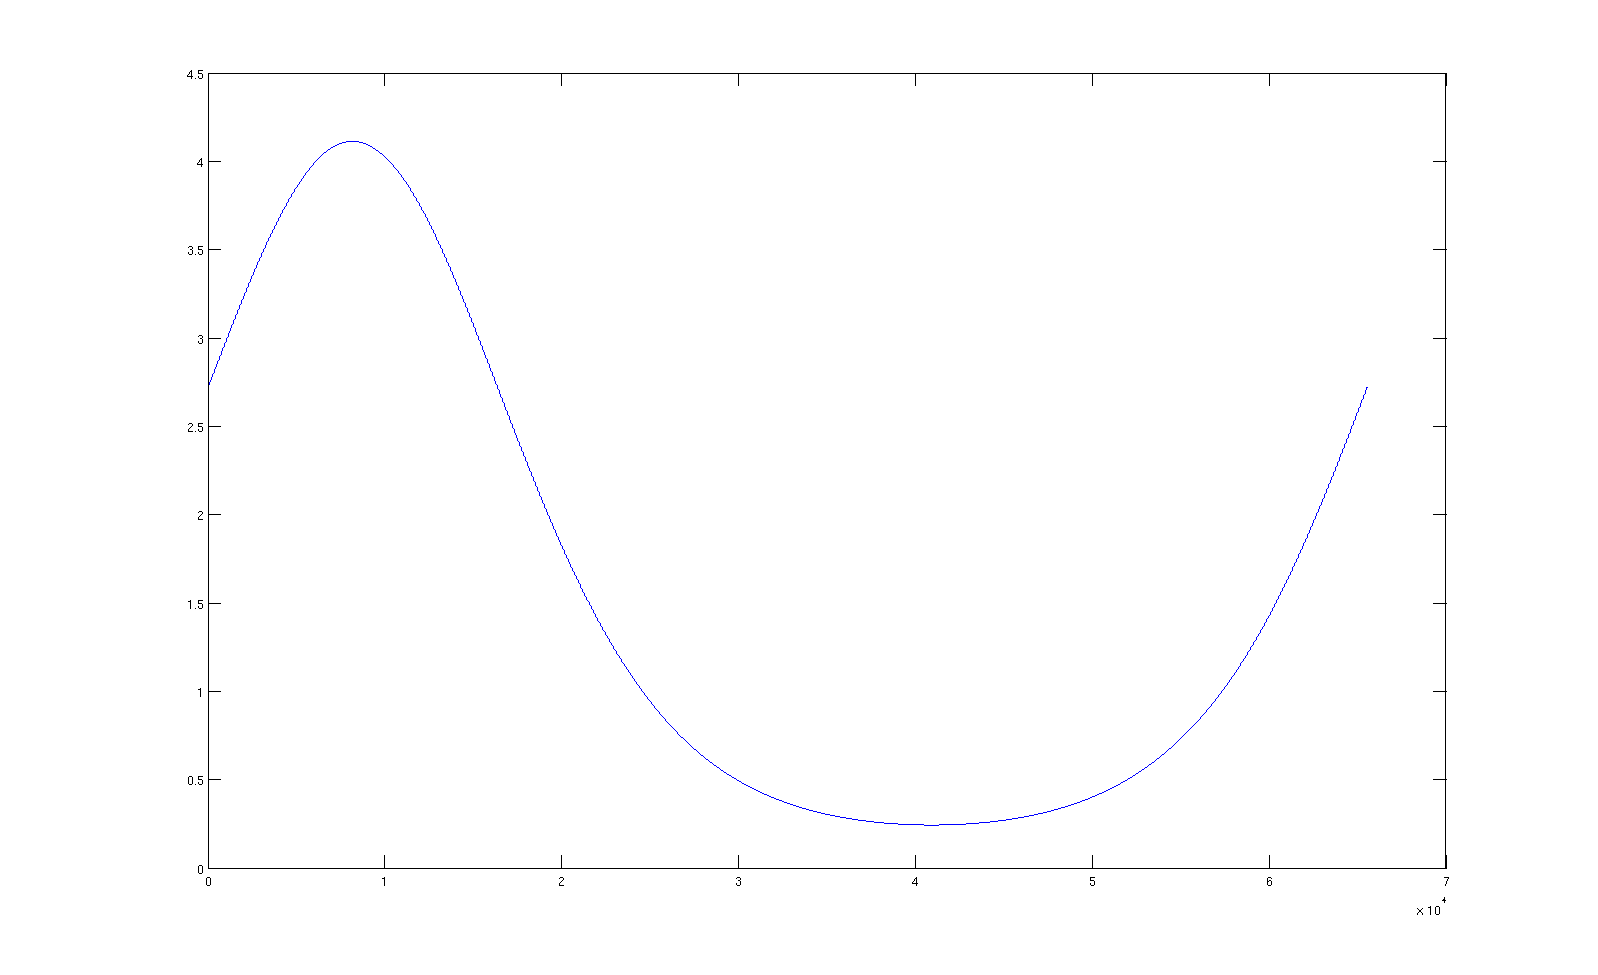
\includegraphics[width=3in]{hw1_part1_fig1.png} & 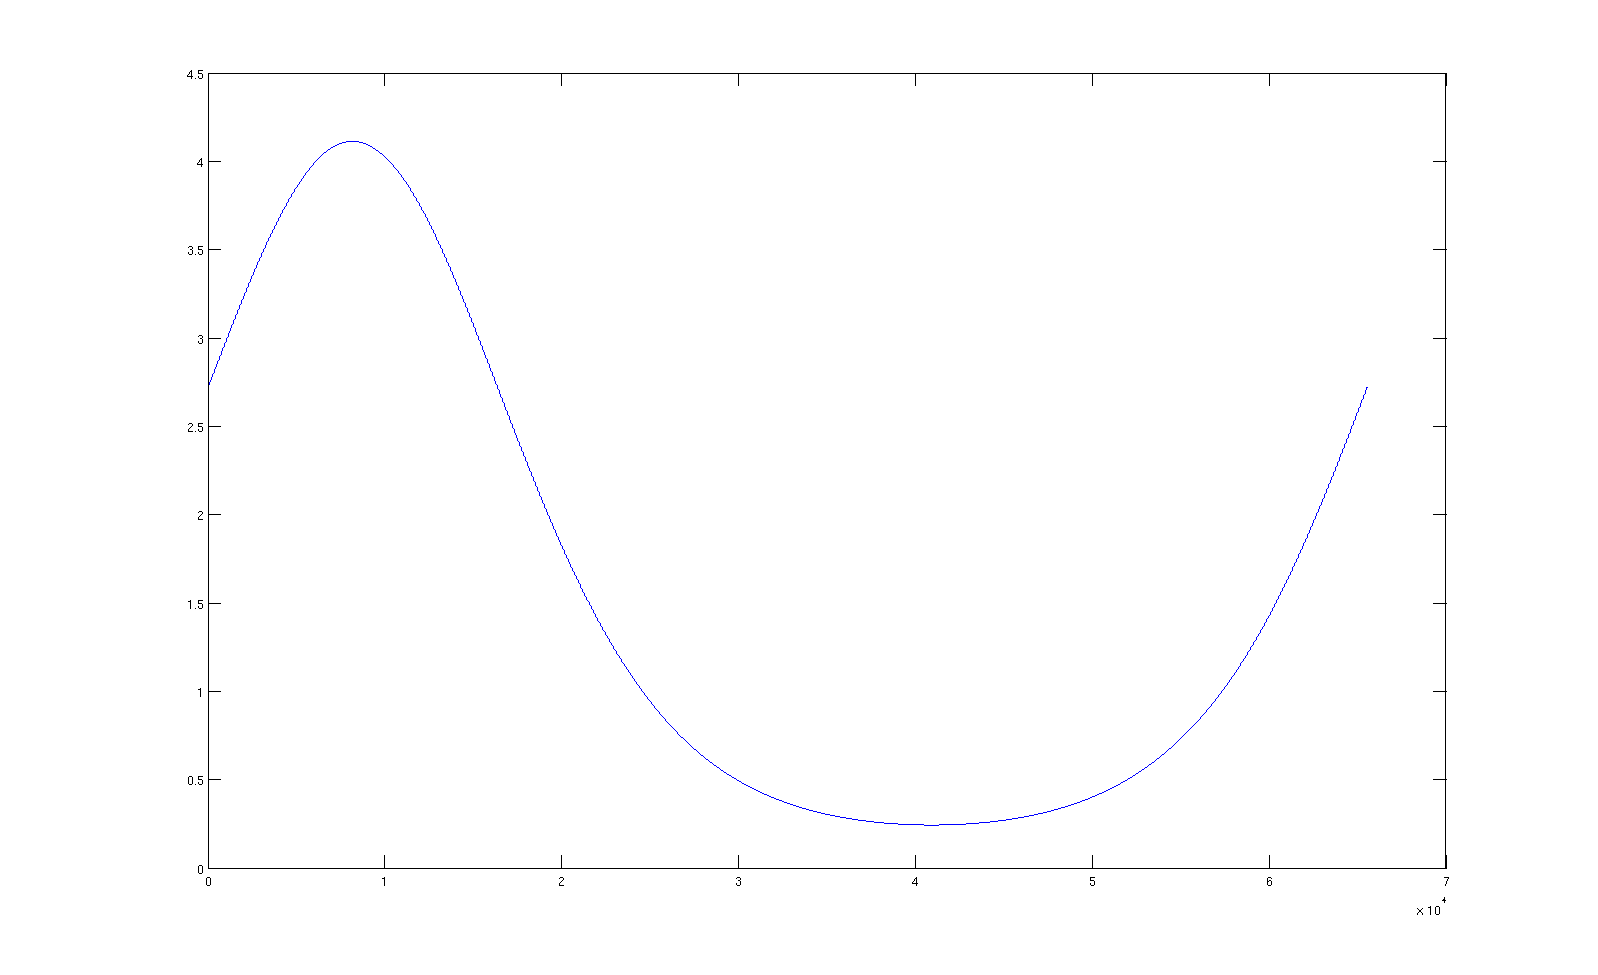
\includegraphics[width=3in]{hw1_part1_fig2.png} \\
Galerkin Solution & Exact Solution \\
\end{tabular}

\paragraph{3}

The following figure shows the RMS error for this method relative to the number of elements:

\begin{center}
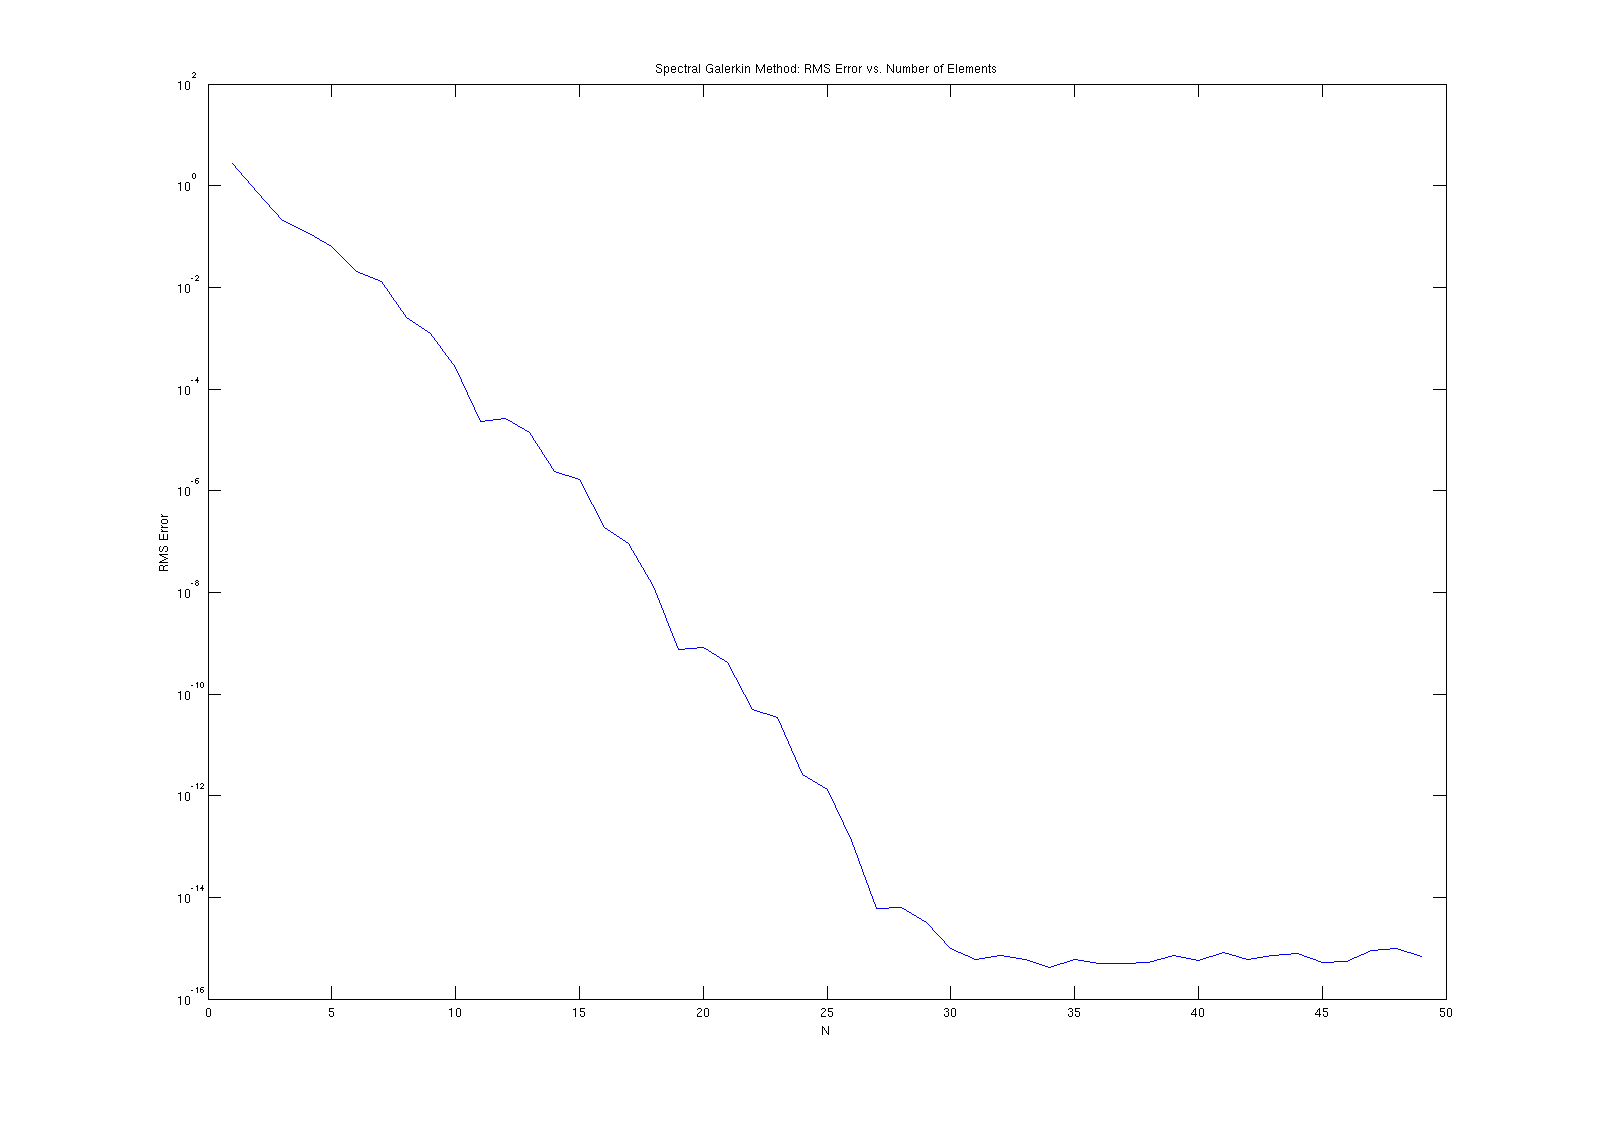
\includegraphics[width=4in]{hw1_part1_fig3.png}
\end{center}

Up to $N \approx 30$, the accuracy of the approximation is on the order of $10^{-N/2}$, at which point the error stabilizes.  This is due to the fact that at this point the precision is on the order of $10^{-15}$ which is the limit of what may be represented within a double.  Beyond this point, any additional fluctuation is simply machine noise.

\paragraph{4}

\subparagraph{a}
\begin{eqnarray*}
\mathcal{F}\{ \lambda(u + v) \}( \omega ) & = & \int \limits_{\mathbb{R}} (\lambda(u(x) + v(x)) e^{-i x k} d x \\
& = & \lambda \int \limits_{U(1)} u(x) e^{-i x k} + v(x) e^{-i x k} dx \\
& = & \lambda \hat{u}(k) + \lambda \hat{v}(k)
\end{eqnarray*}

\subparagraph{b}
\begin{eqnarray*}
\mathcal{F}\{ u(x+x_0) \}(k) &= & \int \limits_{ \mathbb{R} } u(x+x_0) e^{-i x k} d x \\
 & = & \int \limits_{\mathbb{R} } u(x) e^{-i (x + x_0) k} dx \\
 & = & e^{-i x_0 k} \hat{u}(k)
\end{eqnarray*}

\subparagraph{c}
\begin{eqnarray*}
\mathcal{F}\{ e^{i k_0 x}u(x) \}(k) &= & \int \limits_{ \mathbb{R} } u(x) e^{i k_0 x} e^{-i x k} d x \\
 & = & \int \limits_{\mathbb{R} } u(x) e^{-i x (k - k_0} dx \\
 & = & \hat{u}(k - k_0)
\end{eqnarray*}

\subparagraph{d}
\begin{eqnarray*}
\mathcal{F}\{u(cx)\} (k) & = & \int \limits_\mathbb{R} u(c x) e^{-i x k} d x \\
& = & \frac{1}{|c|} \int \limits_{\mathbb{R}} u(x) e^{-i \frac{x k}{c} } dx \\
& = & \frac{1}{|c|} \hat{u}(\frac{k}{c})
\end{eqnarray*}

\subparagraph{e}
\begin{eqnarray*}
\mathcal{F} \{ \overline{u(x)} \} (k) & = & \int \limits_\mathbb{R} \overline{u(x)} e^{-i x k} d x\\
& = & \overline{ \int \limits_\mathbb{R} u(x) e^{i x k} dx } \\
& = & \overline{ \hat{u}(-k) }
\end{eqnarray*}

\subparagraph{f}
\begin{eqnarray*}
\partial_x \left \{ \mathcal{F}^{-1} \mathcal{F}\{ u \}  \right \}(x) & = & \partial_x \left ( \frac{1}{2 \pi}\int \limits_\mathbb{R} \left( \int \limits_\mathbb{R} u(t) e^{-i t k} dt \right) e^{i x k} dk \right) \\
& = & \frac{1}{2 \pi} \int \limits_\mathbb{R} i k  \int \limits_\mathbb{R} u(t) e^{-i t k} dt \: e^{i x k} dk \\
& = & \mathcal{F}^{-1} \{ i k \hat{u} \}
\end{eqnarray*}

\subparagraph{g}
Part f is applied in the last step
\begin{eqnarray*}
\mathcal{F}^{-1} \{ u \} (k) & = & \frac{1}{2 \pi} \int \limits_\mathbb{R} u(x) e^{i x k} dx \\
& = & \frac{1}{2 \pi} \overline{ \int \limits_\mathbb{R} \overline{u(x)} e^{-i x k} d x } \\
& = & \frac{1}{2 \pi} \overline{ \hat{ \overline{u} } (k) } \\
& = & \frac{1}{2 \pi} \hat{u}(-k)
\end{eqnarray*}


\paragraph{5}
Let $K_n$ be the kernel for an $n$-point central finite difference operator with sampling distance $h$.  Then for $n=2,4$ we have:
\begin{eqnarray*}
K_2(x) & = & \frac{1}{2h} \left( \delta(x-h) - \delta(x+h) \right) \\
K_4(x) & = & \frac{1}{12h} \left( -\delta(x-2h) + 8 \delta(x-h) - 8 \delta(x+h) + \delta(x+2h) \right)
\end{eqnarray*}

The corresponding multiplier for $K_n$ is equivalent to taking its Fourier transform:
\[ g_n = \mathcal{F}\{ K_n \} \]

To compute $g_n$, we apply the linearity and translation identities from problem 4, along with the fact that $\mathcal{F}\{\delta\} = \frac{1}{2 \pi}$ and recover the following expression for $g_2, g_4$:
\begin{eqnarray*}
g_2(k) & = & \frac{1}{4 \pi h} \left( e^{-ikh} - e^{ikh} \right) \\
g_4(k) & = & \frac{1}{24 \pi h} \left( -e^{-2ikh} + 8 e^{-ikh} - 8 e^{ikh} + e^{2ikh} \right)
\end{eqnarray*}

Plotting the imaginary component of these multipliers against $g_\infty$ gives the following result:

\begin{center}
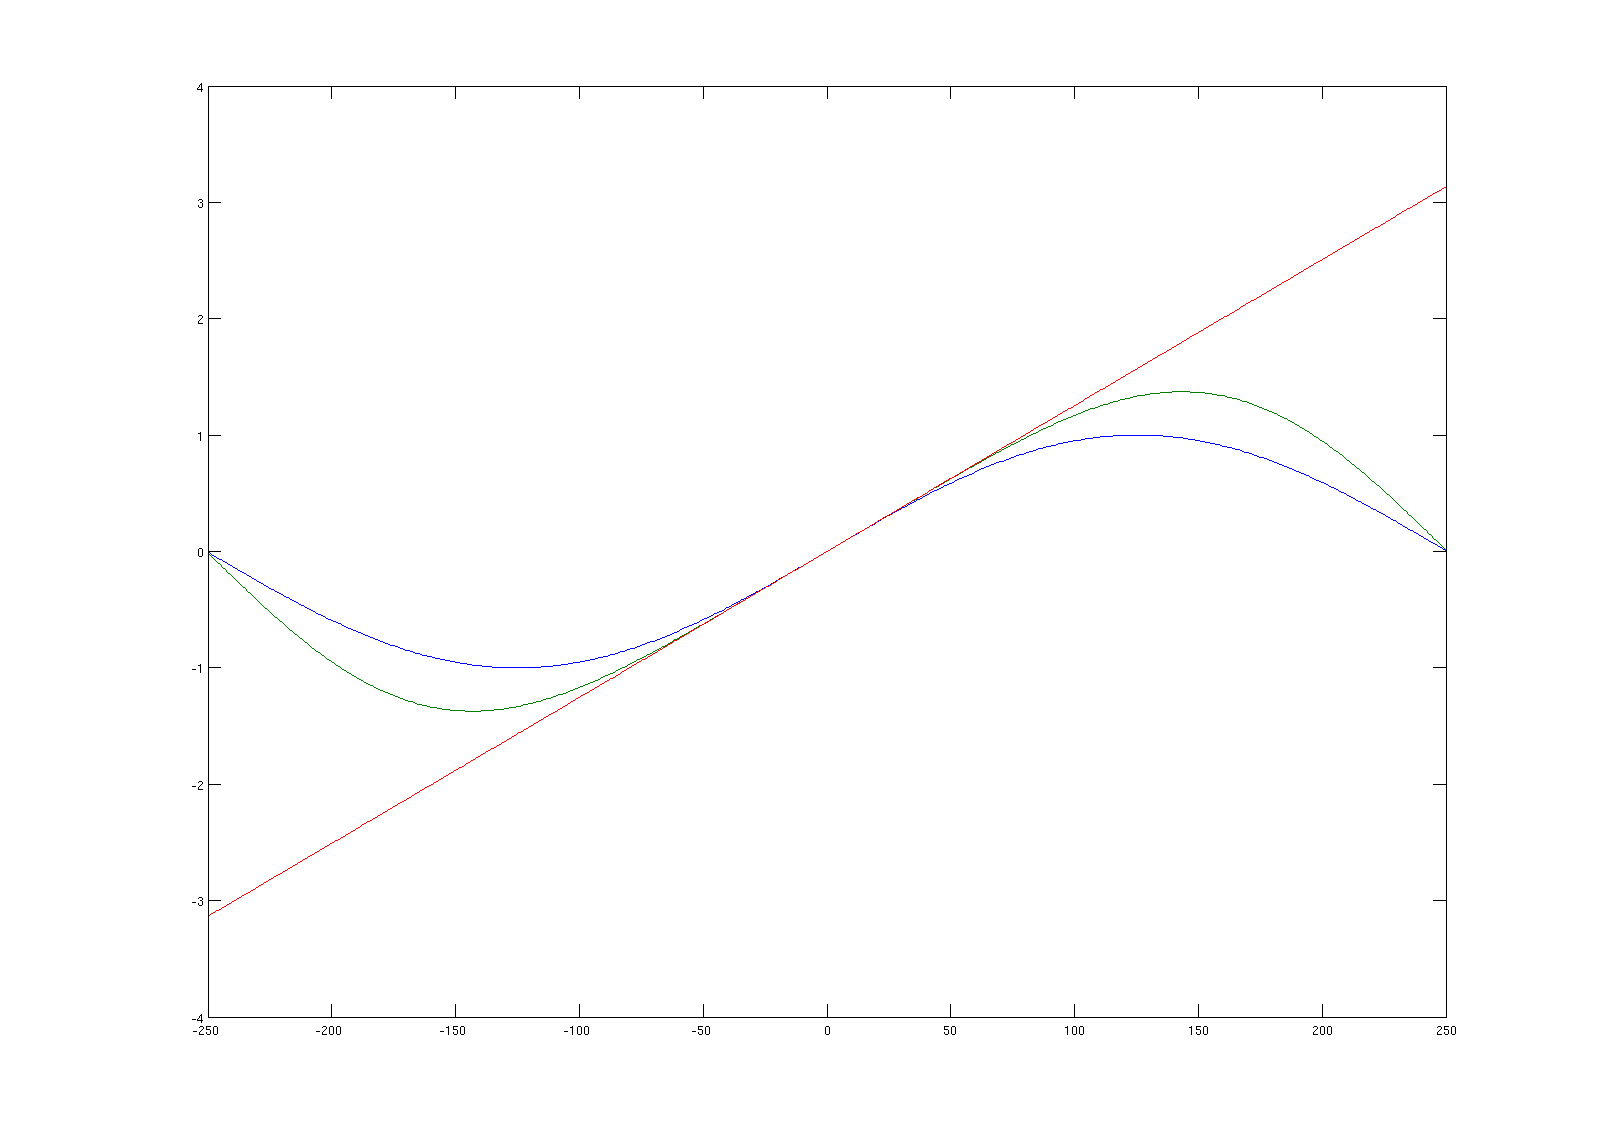
\includegraphics[width=5in]{hw1_p5_fig1.png}
\end{center}

$g_2$ is shown in blue, $g_4$ in green and $g_\infty$ in red.  As the order of accuracy increase, the multipliers approximate the asymptote $g_\infty$ more closely.  Generally, it appears that these operators are more accurate at lower frequencies and become progressively worse as the frequency increases.

\paragraph{6}
\subparagraph{a}
This system is a homogeneous, linear, first-order PDE.  Since the coefficient on $u_t$ is $1$, the characteristic, $\varphi$ curve may be parameterized as a function of $t$ and satisifying the equation:
\[ \frac{d\varphi(t)}{dt} = \frac{1}{5} + \sin^2( \varphi(t) - 1 ) \]
Which can be solved using Mathematica to get:
\[ \varphi(t) = 1-\tan ^{-1}\left(\frac{\tan \left(\frac{\sqrt{6}}{5} \left( C - t \right)\right)}{\sqrt{6}}\right) \]
This function, when substituted into the original PDE has a period of $\frac{10 \pi}{\sqrt{6} } \approx 13$.

\subparagraph{b}

To solve this problem, the code from part a was modified to take a variable time / sampling step as follows:

\begin{verbatim}
function [data] = p6_param(T,N)
  h = 2*pi/N; x = h*(1:N); t = 0; dt = h/4;
  c = .2 + sin(x-1).^2;
  v = exp(-100*(x-1).^2); 

  data = [v];
  vold = exp(-100*(x-.2*dt-1).^2);
  
  for i = 1:floor(T / dt)
      t = t+dt;
      v_hat = fft(v);
      w_hat = 1i*[0:N/2-1 0 -N/2+1:-1] .* v_hat;
      w = real(ifft(w_hat)); 
      vnew = vold + 2*dt*c.*w; 
      vold = v; 
      v = vnew;
      data(i+1,:) = v;
  end
end
\end{verbatim}

From this, it was possible to graph the $L^\infty$ error of the convergence, given the periodicity of the solution:

\begin{center}
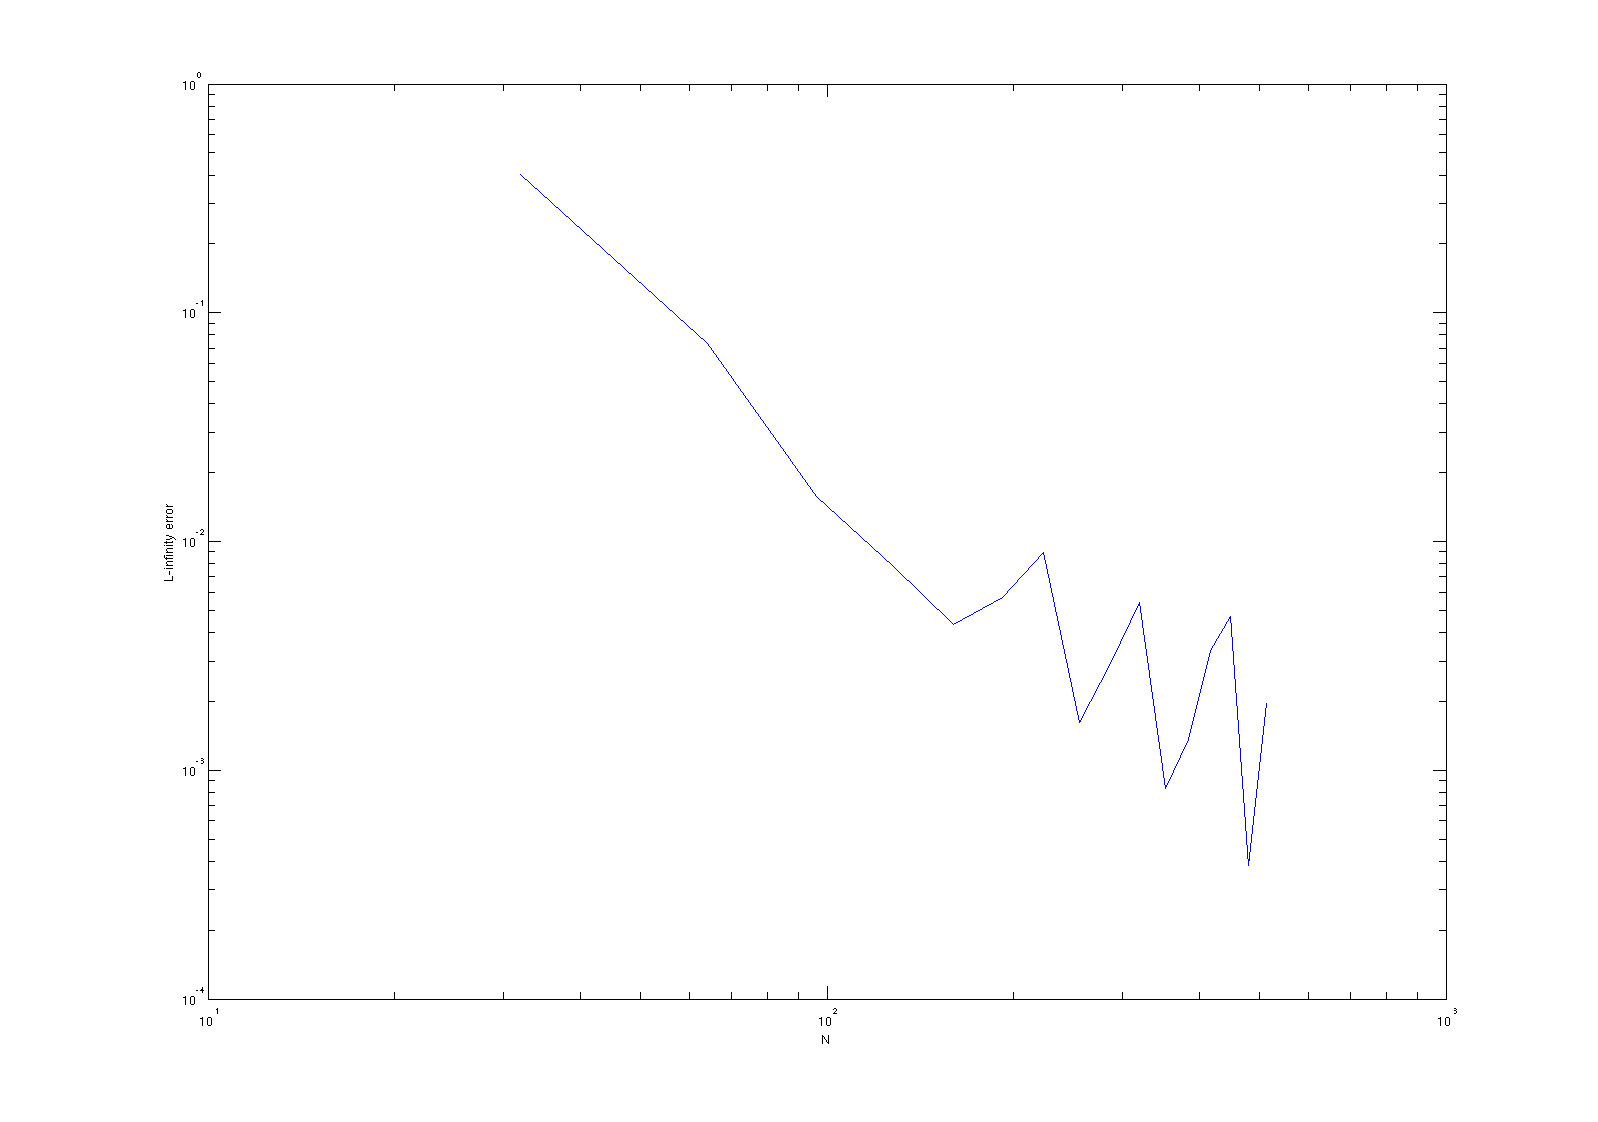
\includegraphics[width=4in]{hw1_part2_p6b.png}
\end{center}

To improve this solution, one could use the exact analytic solution.  This would give the correct answer for arbitrary $t$ and boundary conditions with much less computational effort.

\subparagraph{c}
As we showed at the start of problem 2, the chosen Galerkin approximation for this system is equivalent to the spectral solution up to a change of variables.  Thus, the resulting solution will be the same.

\paragraph{7}

We prove the following lemma which is sufficient to resolve most of the individual cases in theorem 3 (thereby sparing the grader the agony of parsing so much text):

\subparagraph{Lemma}
If $|u| \in O(f(k)) \cap L^2(\mathbb{R})$ with $u$ having first derivative of bounded variation; $f = \partial_k F$ where $f'$ is positive, symmetric, monotonic and $\lim_{k \to \infty}F(k) \to 0$; and $v(j) = u(h j)$ (for $j \in \mathbb{Z}$), then for all $k \in [- \frac{\pi}{h}, \frac{\pi}{h} ]$:
\[ | \hat{v}(k) - \hat{u}(k) | \in O\left( \frac{1}{h} F\left(k + \frac{2 \pi}{h}\right) \right) \]

\subparagraph{Proof}
By theorem 2, we know that:
\[ |\hat{v}(k)| = |\sum \limits_{j=-\infty}^{\infty} \hat{u}(k + \frac{2 \pi j}{h})| \]
Which by the hypothesis is bounded by:
\begin{eqnarray*}
|\hat{v}(k) - \hat{u}(k)| & \leq & C \sum \limits_{j=-\infty, j \neq 0}^{\infty} f \left(k + \frac{2 \pi j}{h} \right) \\
& = & 2C  \sum \limits_{j=1}^{\infty} f \left( k + \frac{2 \pi j}{h} \right) \\
& \leq & C \int \limits_{1}^{\infty} f \left( k + \frac{2 \pi y}{h} \right) dy \\
& \leq & \frac{C}{h} \int \limits_{k + \frac{2 \pi}{h}}^{\infty} f(x) dx \\
& = & \frac{C F \left(k + \frac{2 \pi}{h} \right) } {h}
\end{eqnarray*}

The results in the theorem 3a-c then follow naturally as corrollaries of theorems 1a-c.  For theorem 3d, we take a different approach.  By theorem 1d, we know that $\hat{u}$ has compact support on $[-\alpha, \alpha]$, if $h \leq \frac{\pi}{\alpha}$, then $u$ may be extended to a function, $\hat{u'}$ with period $2\pi$ that agrees exactly with $\hat{u}$ on $[-\pi, \pi]$, such that $\textrm{square}(k) \hat{u'}(k) = \hat{u}(k)$.  Thus, $\textrm{sinc}(\frac{x}{h}) \star u'(x) = u(x)$.  However, convolution with $\textrm{sinc}(\frac{x}{h})$ fixes all points at $h \mathbb{Z}$, and thus agrees with $u'(h j) = u(h j) = v(j)$.  Therefore, the transformation is exact.

\paragraph{8}
We consider both the cases $m=2,4$ using the same approach.  In each case, the graph shows a log-plot of the $L^2$ norm of the difference between subsequent eigenvalue approximations (with respect to the grid size, $N$).  The tables consist of the Eigen values computed up to 10-digit accuracy.

\begin{center}
\begin{tabular}{cc}
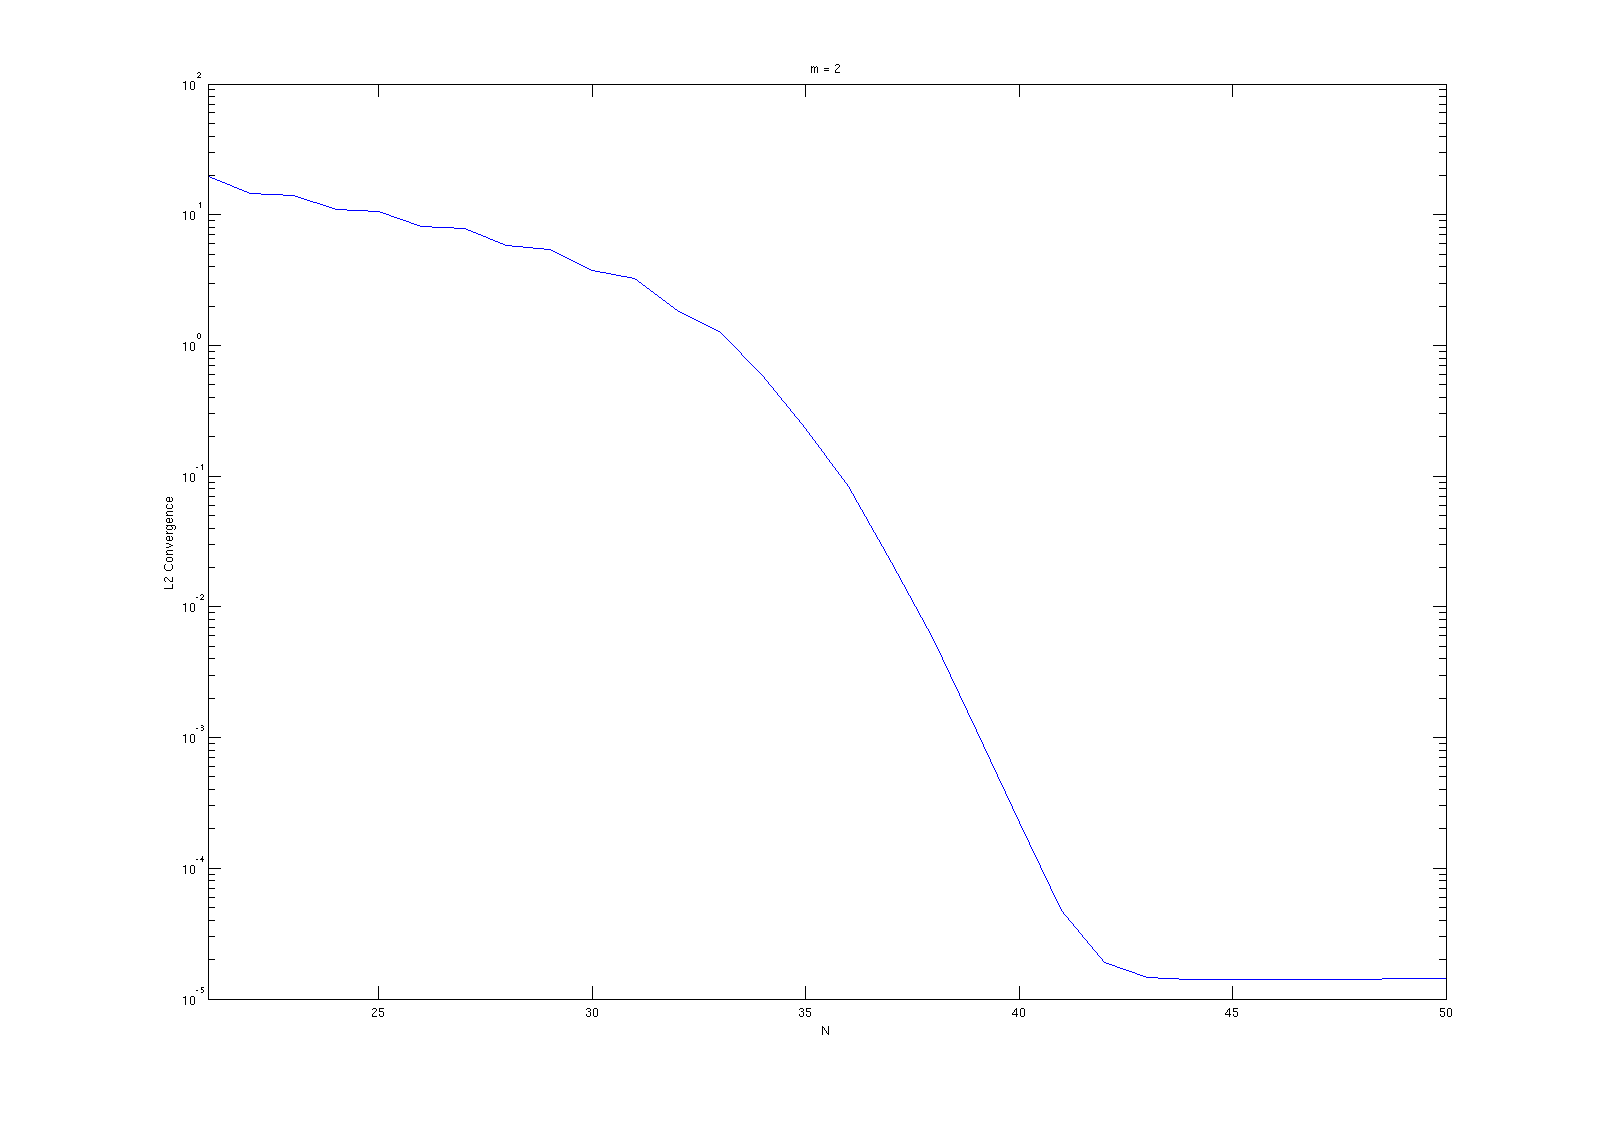
\includegraphics[width=3.5in]{hw1_part2_p8_fig1.png} & 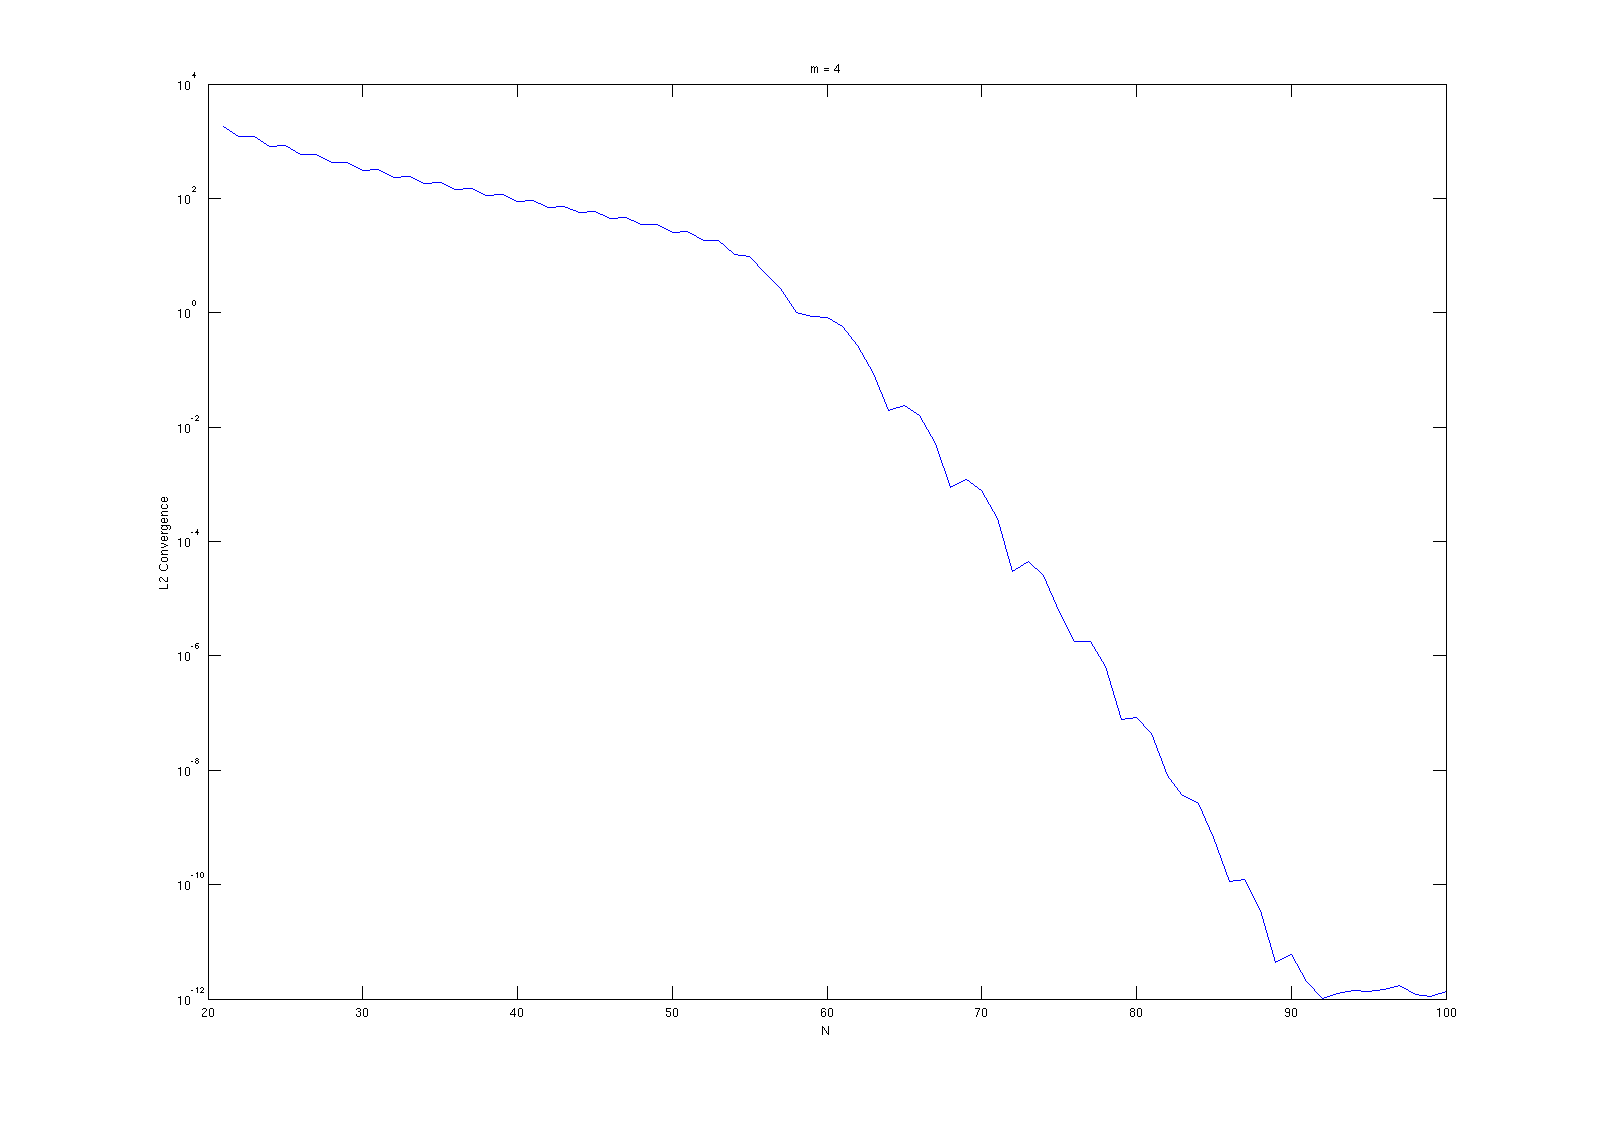
\includegraphics[width=3.5in]{hw1_part2_p8_fig2.png} \\
L2 Convergence, $m=2$ & L2 Convergence, $m=4$ \\
\end{tabular}
\end{center}

\begin{center}
\begin{tabular}{|c|c|}
\hline
m = 2 & m = 4 \\
\hline
   1.000000000000032 &  1.060362090484225 \\
   2.999999999999991 &	3.799673029801529 \\
   4.999999999999835 &  7.455697937986940 \\
   6.999999999999964 &  11.644745511378069  \\
   9.000000000000028 &  16.261826018850122 \\
  10.999999999999845 &  21.238372918235811 \\
  13.000000000000020 &  26.528471183682196 \\
  14.999999999999911 &  32.098597710968413 \\
  16.999999999999982 &  37.923001027034573 \\
  18.999999999999964 &  43.981158097289978 \\
  20.999999999999591 &  50.256254516682972 \\
  23.000000000003396 &  56.734214055173275 \\
  24.999999999969774 &  63.403046986718707 \\
  27.000000000227086 &  70.252394628616571 \\
  28.999999998365411 &  77.273200481983679 \\
  31.000000010109567 &  84.457466274941694 \\
  32.999999939015886 &  91.798066808991138 \\
  35.000000313583499 &  99.288606660493429 \\
  36.999998392438492 & 106.9233073817323 \\
  39.000006910394958 & 114.6969173849852 \\
\hline
\end{tabular}
\end{center}

To compute these results, the following modified version of the linked code was used:

\begin{verbatim}
function [ res ] = p8_param( N, m )
  L = 8;                            
  h = 2*pi/N; x = h*(1:N); x = L*(x-pi)/pi;
  column = [-pi^2/(3*h^2)-1/6 ...
      -.5*(-1).^(1:N-1)./sin(h*(1:N-1)/2).^2];
  D2 = (pi/L)^2*toeplitz(column); 
  eigenvalues = sort(eig(-D2 + diag(x.^m)));
  res = eigenvalues(1:20);
end
\end{verbatim}

Program wise, the main change in the code from the case where $m=2$ to $m=4$ is that the exponent on the diagonal matrix has to change.  Otherwise, the same procedure works in both cases.  In terms of the convergence, it should be noted that the $m=4$ case converged much more slowly.  Overall, it took nearly twice as many samples as the $m=2$ case to reach a similarly stable state.

\end{document}

